\phantomsection
\section{INSAT-3D SRF Data Plots}
%================================
\label{app.srf_data_plots}

\subsection{Imager}
%------------------

\begin{figure}[H]
  \centering
  \begin{tabular}{c c}
    \includegraphics[scale=0.35]{graphics/imgr/srf/imgr_insat3d-3.eps} &
    \includegraphics[scale=0.35]{graphics/imgr/srf/imgr_insat3d-4.eps} \\
    \includegraphics[scale=0.35]{graphics/imgr/srf/imgr_insat3d-5.eps} &
    \includegraphics[scale=0.35]{graphics/imgr/srf/imgr_insat3d-6.eps}
  \end{tabular}
  \caption{INSAT-3D Imager channels 3-6 spectral responses. Vertical dashed lines are the locations of the computed central frequencies.}
  \label{fig:imgr_ch3-6}
\end{figure}


\subsection{Sounder}
%------------------

\addcontentsline{toc}{subsubsection}{Channels 1-6}
\begin{figure}[H]
  \centering
  \begin{tabular}{c c}
    \includegraphics[scale=0.35]{graphics/sndr/srf/sndr_insat3d-1.eps} &
    \includegraphics[scale=0.35]{graphics/sndr/srf/sndr_insat3d-2.eps} \\
    \includegraphics[scale=0.35]{graphics/sndr/srf/sndr_insat3d-3.eps} &
    \includegraphics[scale=0.35]{graphics/sndr/srf/sndr_insat3d-4.eps} \\
    \includegraphics[scale=0.35]{graphics/sndr/srf/sndr_insat3d-5.eps} &
    \includegraphics[scale=0.35]{graphics/sndr/srf/sndr_insat3d-6.eps}
  \end{tabular}
  \caption{INSAT-3D Sounder channels 1-6 spectral responses. Vertical dashed lines are the locations of the computed central frequencies.}
  \label{fig:sndr_ch1-6}
\end{figure}

\addcontentsline{toc}{subsubsection}{Channels 7-12}
\begin{figure}[H]
  \centering
  \begin{tabular}{c c}
    \includegraphics[scale=0.35]{graphics/sndr/srf/sndr_insat3d-7.eps} &
    \includegraphics[scale=0.35]{graphics/sndr/srf/sndr_insat3d-8.eps} \\
    \includegraphics[scale=0.35]{graphics/sndr/srf/sndr_insat3d-9.eps} &
    \includegraphics[scale=0.35]{graphics/sndr/srf/sndr_insat3d-10.eps} \\
    \includegraphics[scale=0.35]{graphics/sndr/srf/sndr_insat3d-11.eps} &
    \includegraphics[scale=0.35]{graphics/sndr/srf/sndr_insat3d-12.eps}
  \end{tabular}
  \caption{INSAT-3D Sounder channels 7-12 spectral responses. Vertical dashed lines are the locations of the computed central frequencies.}
  \label{fig:sndr_ch7-12}
\end{figure}

\addcontentsline{toc}{subsubsection}{Channels 13-18}
\begin{figure}[H]
  \centering
  \begin{tabular}{c c}
    \includegraphics[scale=0.35]{graphics/sndr/srf/sndr_insat3d-13.eps} &
    \includegraphics[scale=0.35]{graphics/sndr/srf/sndr_insat3d-14.eps} \\
    \includegraphics[scale=0.35]{graphics/sndr/srf/sndr_insat3d-15.eps} &
    \includegraphics[scale=0.35]{graphics/sndr/srf/sndr_insat3d-16.eps} \\
    \includegraphics[scale=0.35]{graphics/sndr/srf/sndr_insat3d-17.eps} &
    \includegraphics[scale=0.35]{graphics/sndr/srf/sndr_insat3d-18.eps}
  \end{tabular}
  \caption{INSAT-3D Sounder channels 13-18 spectral responses. Vertical dashed lines are the locations of the computed central frequencies.}
  \label{fig:sndr_ch13-18}
\end{figure}
